\chapter{Progress to Date}

\section{Rotterdam Longitudinal Glaucomatous \ac{VF} Dataset}

The Longitudinal Glaucomatous Visual Field data from Rotterdam Ophthalmic Data Repository \cite{Bryan2013} consists of data from $139$ patients' $278$ eyes. A total of $4863$ 24-2 test results with MD are available. On average each eye has $17.5$ fields available with mean follow-up time of $9.2$ years. $270$ $(97.1\%)$ eyes have at least $14$ fields with a minimum of $7.6$ years of follow-up. The mean and median follow-up interval between tests is $203$ and $189$ days; the standard deviation of follow-up time is $72.3$ days. $346$ $(7.5\%)$ of follow-ups had an interval of more than $270$ days. 

\subsection{Data Characteristics}

To investigate the composition of healthy versus glaucomatous patients the dataset, the characteristic of MD values in the dataset is investigated. In figure \ref{fig:mean_md_hist} the distribution of average MD value calculated from all tests administers on an eye for each of the $278$ eyes is shown. The mean and median of the distribution are $-8.9$ and $-6.8$ dB respectively. The data set contains mostly eyes with mild to moderate reduced MD values ($75\%$ of eyes have average MD $>-13.2$ dB).

\begin{figure}[h]
	\centering
	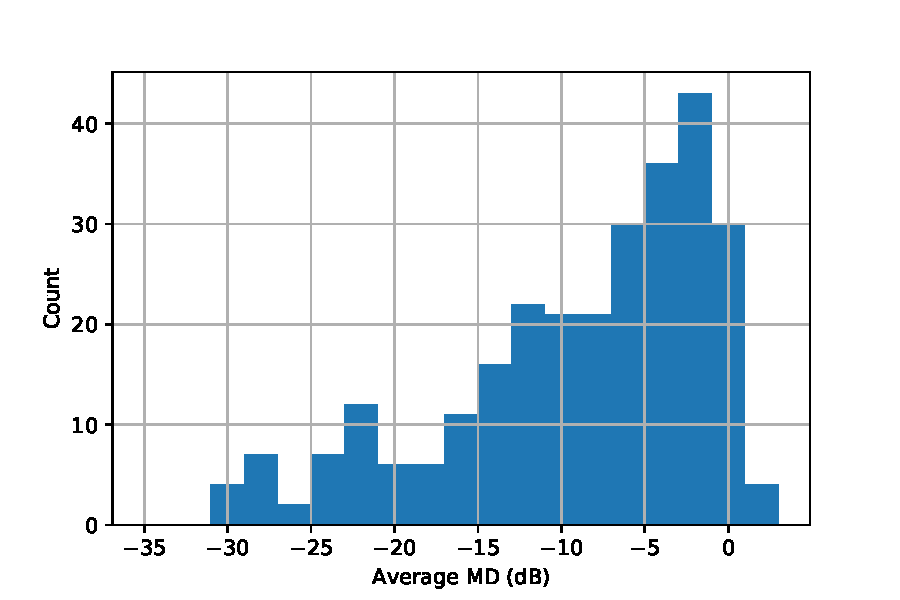
\includegraphics[width=0.6\textwidth]{mean_md_hist}	\caption{Distribution of eyes' average MD values within the Rotterdam dataset ($n=278$)}
	\label{fig:mean_md_hist}
\end{figure}
%
%\begin{figure}[h]
%	\centering
%	\begin{subfigure}[b]{0.45\textwidth}
%		\centering
%		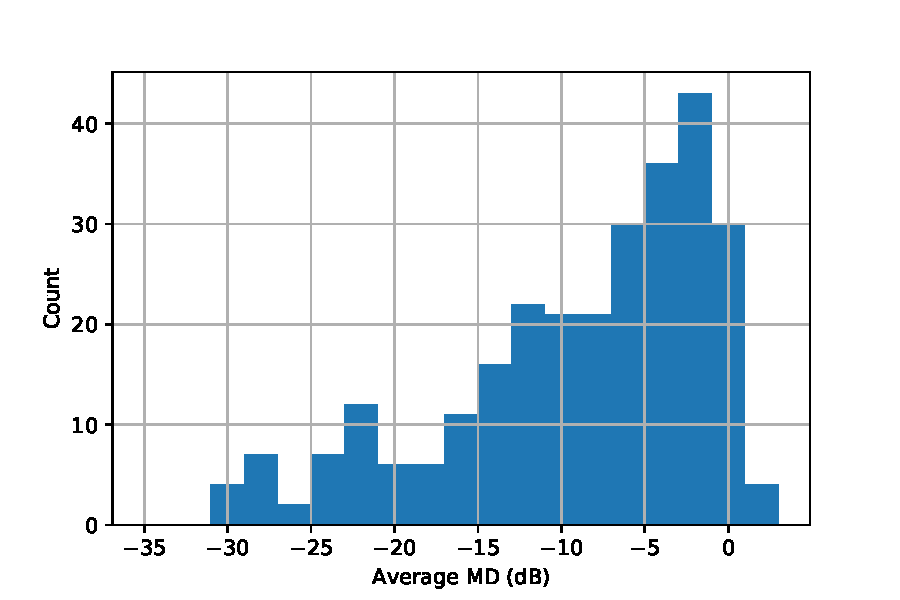
\includegraphics[width=\textwidth]{mean_md_hist}
%		\caption{}
%		\label{fig:mean_md_hist}
%	\end{subfigure}
%	\hfill
%	\begin{subfigure}[b]{0.45\textwidth}
%		\centering
%		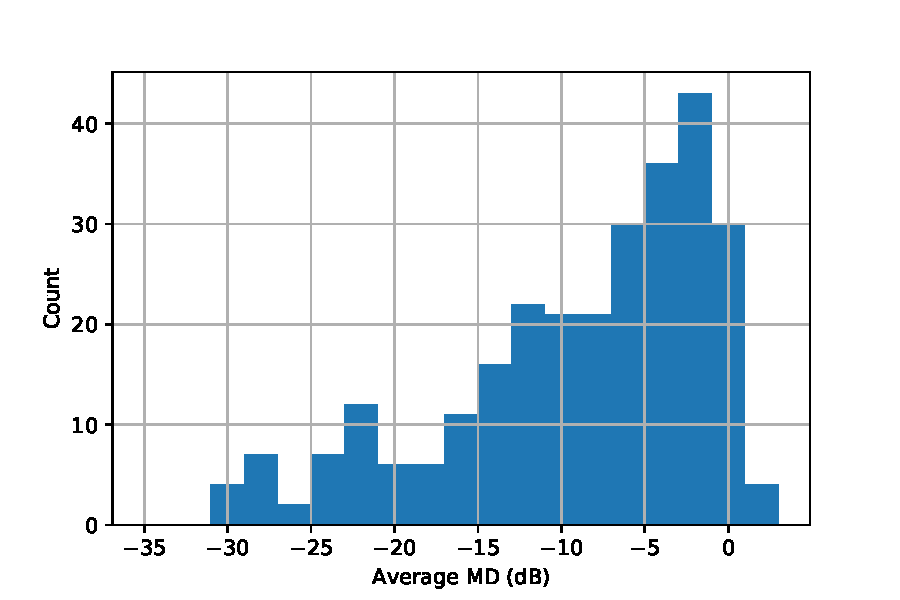
\includegraphics[width=\textwidth]{mean_md_hist}
%		\caption{}
%		\label{fig:three sin x}
%	\end{subfigure}
%	\caption{(a) Distribution of MD values within the patient dataset}
%	\label{fig:study_site}
%\end{figure}
%
%
%
%
